\scanpage{101}
On supposera dorénavant qu'on a \deleted{l'axi.}

\noindent\vrule\hspace{.5em}\begin{minipage}{.89\linewidth}\uline{Axiome 3} \quad Les $\widetilde E_\alpha$ $(\alpha\in t_0)$ sont $\ne\varnothing$, i.e. on n'est pas dans le cas \inserted{(trivial)} envisagé dans la NB précédente, $\unsure{\Leftrightarrow|{=}}$ ou encore : par tt sommet $s\in S$ passent au moins 2 triangles.\end{minipage}

Il reste exprimer dans ce cas, l'axiome 2 pour les triangles sup. Or il est automatique !

\diagram{\begin{tikzcd}[ampersand replacement=\&,row sep=.5em,column sep=.5em]
{}\& s\arrow[dl,dash]\arrow[dr,dash]\arrow[dd,dash]\&{}\\
t\arrow[rr,dash]\arrow[dd,dash]\&{}\&u\arrow[dd,dash]\\
{}\&a\arrow[dl,dash]\arrow[dr,dash]\&{}\\
b\arrow[rr,dash]\&{}\&c
\end{tikzcd}}
\deleted{\uline{Prop} 6 \quad Soit $\{s,t,u\}$ sur $\{a,b,c\}=t_0$ un triangle supérieur (i.e. un $t\in\widetilde\Gamma$), et soit $s_1\in\overline E_a\setminus\{s,s'=\sigma_a s\}$. Alors $s_1$ est lié à $t$ ou $u$ (NB bien sûr, pas aux \uline{deux} à la fois\ldots.)}

En effet, \deleted{\unsure{tout}} a) tt $\alpha\in t_0$ est lié à un pt de $\{s,t,u\}$

\deleted{\unsure{$s$ distinct} \unsure{et|de}} b) Si $\deleted{\unsure{a}}s_1\in\deleted{E_\alpha,\ \text{alors}}S\setminus t_0=\coprod\overline E_\alpha$, disons $s_1\in E_a$, \deleted{pour $\alpha\in t_0$ \unsure{conv.}, alors} $s_1\notin t$ i.e. $s_1\ne s$, si $s_1$ \deleted{$=\sigma_\alpha s=s'$, il est} n'est pas lié à $s$ i.e. $s_1\ne s'=\sigma_a s$, montrons qu'il est lié à $t$ ou $u$. En effet, s'il n'était lié à aucun des deux, alors $s'_1=\sigma_\alpha s_1$ serait lié aux deux à la fois, et comme $s'_1\ne s$ c'est absurde.

\par\centerline{\rule{4cm}{.4pt}}

\uline{\unsure{Rescholie|Résolution}}

En résumé, la donnée d'un complexe $(S,A)$ \deleted{\unsure{entier|et \illegible{1}}} satisfaisant les axiomes \textcircled{1}, \textcircled{\unsure{2|1}} et qui n'est pas du type trivial \deleted{\unsure{étudié|étoile}} \inserted{(\unsure{discret|disons}, se réduisant à un triangle, ou à une étoile de triangles
\figure{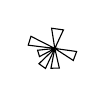
\begin{tikzpicture}[scale=.20]\foreach \a/\b/\r in {65/99/1.3,153/173/1.7,186/208/1.1,224/245/1.4,259/283/1.28,327/352/1.4}{\draw (0,0)--(\a:\r)--(\b:\r)--cycle;}\end{tikzpicture}})} équivaut à celle de
% archive sheet number: 100
